\documentclass[tikz,border=4pt]{standalone}
\usepackage{tikz}
\usetikzlibrary{positioning, arrows.meta, decorations.pathreplacing, calc}
\usepackage{amsmath}
\usepackage{times}       % Times New Roman — IEEE approved font
\usepackage{helvet}      % Helvetica for sans-serif — IEEE approved font
\usepackage{mathptmx}    % Times in math mode

\begin{document}
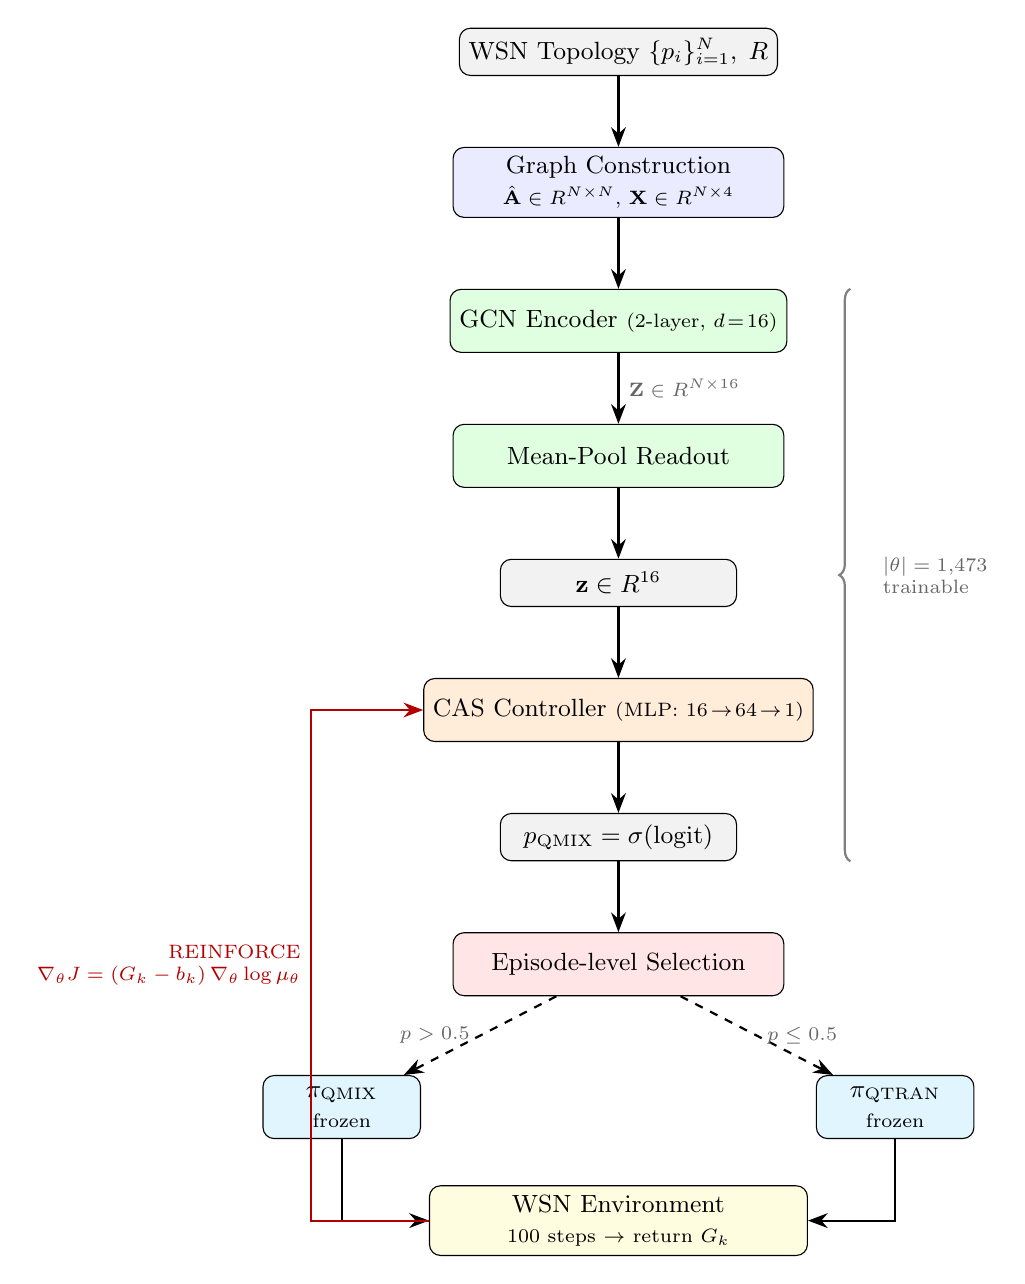
\begin{tikzpicture}[
    node distance=0.9cm,
    box/.style={draw, rounded corners, minimum height=0.8cm, minimum width=4.2cm, align=center, font=\small},
    data/.style={draw, rounded corners, minimum height=0.6cm, minimum width=3.0cm, align=center, fill=gray!10, font=\small},
    arrow/.style={-{Stealth[length=2.5mm]}, thick},
    dasharrow/.style={-{Stealth[length=2.5mm]}, thick, dashed},
    label/.style={font=\scriptsize, text=black!60},
]
\node[data] (topo) {WSN Topology $\{p_i\}_{i=1}^N,\; R$};
\node[box, below=of topo, fill=blue!8] (graph) {Graph Construction\\{\scriptsize $\hat{\mathbf{A}} \in \mathbb{R}^{N \times N}$, $\mathbf{X} \in \mathbb{R}^{N \times 4}$}};
\node[box, below=of graph, fill=green!12] (gcn) {GCN Encoder {\scriptsize (2-layer, $d\!=\!16$)}};
\node[box, below=of gcn, fill=green!12] (pool) {Mean-Pool Readout};
\node[data, below=of pool] (embed) {$\mathbf{z} \in \mathbb{R}^{16}$};
\node[box, below=of embed, fill=orange!15] (cas) {CAS Controller {\scriptsize (MLP: $16 \!\to\! 64 \!\to\! 1$)}};
\node[data, below=of cas] (prob) {$p_{\text{QMIX}} = \sigma(\text{logit})$};
\node[box, below=of prob, fill=red!10] (decision) {Episode-level Selection};
\node[box, below left=1.0cm and 0.4cm of decision, fill=cyan!12, minimum width=2.0cm] (qmix) {$\pi_{\text{QMIX}}$\\{\scriptsize frozen}};
\node[box, below right=1.0cm and 0.4cm of decision, fill=cyan!12, minimum width=2.0cm] (qtran) {$\pi_{\text{QTRAN}}$\\{\scriptsize frozen}};
\node[box, below=2.4cm of decision, fill=yellow!12, minimum width=4.8cm] (env) {WSN Environment\\{\scriptsize 100 steps $\to$ return $G_k$}};
\draw[arrow] (topo) -- (graph);
\draw[arrow] (graph) -- (gcn);
\draw[arrow] (gcn) -- node[right, label] {$\mathbf{Z} \in \mathbb{R}^{N \times 16}$} (pool);
\draw[arrow] (pool) -- (embed);
\draw[arrow] (embed) -- (cas);
\draw[arrow] (cas) -- (prob);
\draw[arrow] (prob) -- (decision);
\draw[dasharrow] (decision) -- node[left, label] {$p > 0.5$} (qmix);
\draw[dasharrow] (decision) -- node[right, label] {$p \leq 0.5$} (qtran);
\draw[arrow] (qmix) |- (env);
\draw[arrow] (qtran) |- (env);
\draw[arrow, red!70!black, thick]
    (env.west) -- ++(-1.5, 0) |- (cas.west)
    node[pos=0.25, left, font=\scriptsize, text=red!70!black, align=right]
    {REINFORCE\\$\nabla_\theta J = (G_k - b_k)\,\nabla_\theta \log \mu_\theta$};
\draw[decorate, decoration={brace, amplitude=4pt, mirror}, thick, black!50]
    let \p1=(gcn.north east), \p2=(prob.south east) in
    (\x1+0.8cm, \y1) -- (\x1+0.8cm, \y2)
    node[midway, right=8pt, font=\scriptsize, text=black!60, align=left] 
    {$|\theta| = 1{,}473$\\trainable};
\end{tikzpicture}
\end{document}
